% \begin{figure}[!t]
%     \centering
%     \includegraphics[width=0.7\linewidth]{figures/moa_illustration.pdf}
%     \caption{Fine-tune LLM with dynamic adapters.}
%     \label{fig:moa_illustration}
% \end{figure}

\section{Background and Motivation}

% \begin{table*}[!h]
%     \centering
%     \caption{Inference cost of different dynamic adapters.}
%     \label{table:moa_latency}
%     \begin{tabular}{lccc}
%     \toprule
%     Method & Decoding latency (ms/token) & Parameter size (B) & FLOPS (G) \\
%     \midrule
%     Llama2-7B  & 2.4 & 6.74 & 6.61 \\
%     MOLA~\cite{gao2024higher} & 25.3 (+954\%) & 7.07(+4.89\%) & 6.65(+0.61\%) \\
%     PESC~\cite{wu2024parameter} & 8.5 (+254\%) & 6.97(+3.41\%) & 6.64(+0.45\%) \\
%     MoRAL~\cite{yang2024moral} & 8.6 (+258\%) & 6.97(+3.41\%) & 6.67(+0.91\%)\\
%     \bottomrule
%     \end{tabular}
% \end{table*}

\begin{table*}[t]
    \centering
    % 移除 \small，保持默认 10pt 字体，符合 AAAI "Table fonts" 建议
    % 如果表格太宽超出页面，可以解除下方 \small 的注释
    % \small 
    
    \begin{tabular}{lccc}
    \toprule
    Method & Decoding latency (ms/token) & Parameter size (B) & FLOPS (G) \\
    \midrule
    Llama2-7B  & 2.4 & 6.74 & 6.61 \\
    MOLA~\cite{gao2024higher} & 25.3 (+954\%) & 7.07 (+4.89\%) & 6.65 (+0.61\%) \\
    PESC~\cite{wu2024parameter} & 8.5 (+254\%) & 6.97 (+3.41\%) & 6.64 (+0.45\%) \\
    MoRAL~\cite{yang2024moral} & 8.6 (+258\%) & 6.97 (+3.41\%) & 6.67 (+0.91\%) \\
    \bottomrule
    \end{tabular}
    
    % Caption 必须在 tabular 之后
    \caption{Inference cost of different dynamic adapters.}
    \label{table:moa_latency}
\end{table*}

% \subsection{Dynamic Adapters}
\noindent\textbf{Dynamic Adapters.}
Given the strengths of both the Mixture of Experts (MoE)~\cite{jiang2024mixtral,artic2024,dbrx2024,xAI-2024} and Low-Rank Adaptation (LoRA)~\cite{Hu2021LoRALA}, their integration has become a focal point of recent research efforts. Recent studies~\cite{feng2024mixtureofloras,gao2024higher,gou2024mixture,liu2023moelora,luo2024moelora} have explored combining these two techniques to further augment the capabilities of large language models (LLMs). This integration leverages the scalability of MoE and the efficiency of LoRA, proposing a promising pathway to meet the escalating demands for model performance and efficiency. 

Formally, the computation process of dynamic adapters can be formulated as:
\begin{align}
    y^l = f^l(x^l) + \sum_{i = 1}^{N}{G^l(x^l)_iE^l_i(x^l)},
    \label{eq:moa_origin}
\end{align}
where the superscript $l$ means $l$-th layer, $N$ represents number of adapters experts, $G^l(x^l) = \text{Softmax}(\text{TopK}(W^l_gx^l))$ represents the top-k (typically top-2) router in the dynamic adapters block, $f^l$ represents the pretrained backbone in $l$-th layer, and $E^l(x^l) = W^l_{up}(W^l_{down}(x^l))$ represents the output of LoRA experts.

Despite an increase in parameters, the experts of the dynamic adapters are activated sparsely, implying that only a limited subset of experts is used per input token. This sparse activation mechanism maintains computational efficiency while significantly expanding the model's capacity to handle diverse scenarios.

% \subsection{Unexpected Latency Overhead of Dynamic Adapters}
\noindent\textbf{Unexpected Latency Overhead of Dynamic Adapters.}
Although dynamic adapters can enhance accuracy and involve only a modest increase in parameter size and computing complexity, they unfortunately introduce a substantial inference latency overhead. We evaluate different dynamic adapter methods with Llama2-7B~\cite{touvron2023llama} on the ShareGPT~\cite{openchat2023sharegpt4} dataset for 50 queries one by one, and generate 200 new tokens for each query. As demonstrated in Table~\ref{table:moa_latency}, existing methods involving dynamic adapters result in an approximate 1\%-5\% increase in parameter count and less than a 1\% increase in computing complexity measured in FLOPS. However, these enhancements lead to a substantial increase in decoding latency, with overheads ranging from 200\% to 950\%.

% \begin{figure}[!h]
%     \centering
%     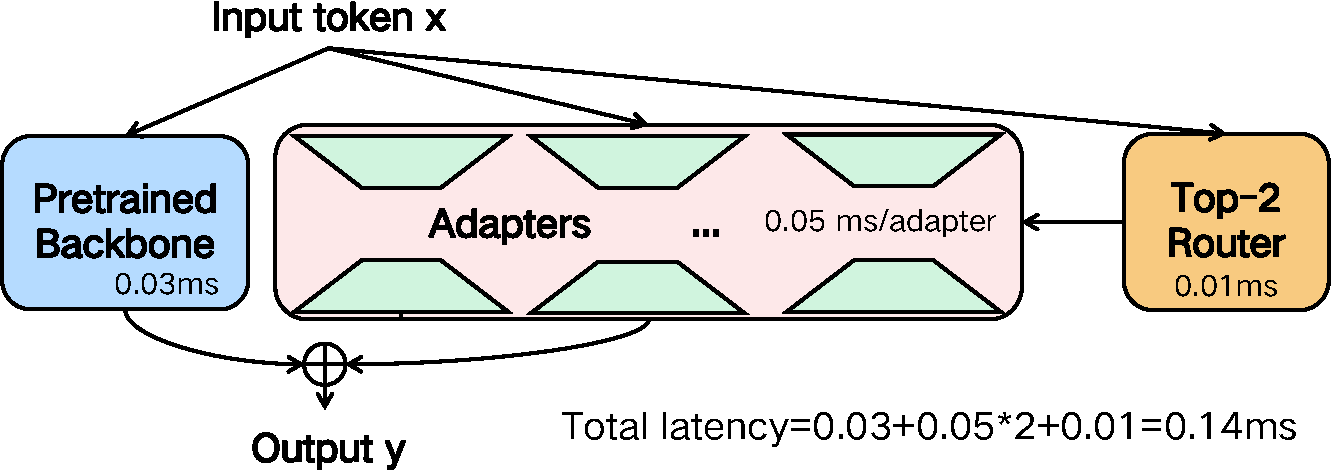
\includegraphics[width=0.49\textwidth]{figures/adapter_latency.pdf}
%     \caption{Decoding phase execution time profiling of one dynamic adapter layer in MoRAL. The execution time results were preceded by a warm-up of 100 executions and are obtained on the average of 300 executions.}
%     \label{fig:cuda_launch}
% \end{figure}

\begin{figure}[t]  % 1. 改为 [t]，强制置顶，符合编辑要求
    \centering
    % 2. 改为 \columnwidth，并设为 0.98 倍以留出一点安全距离
    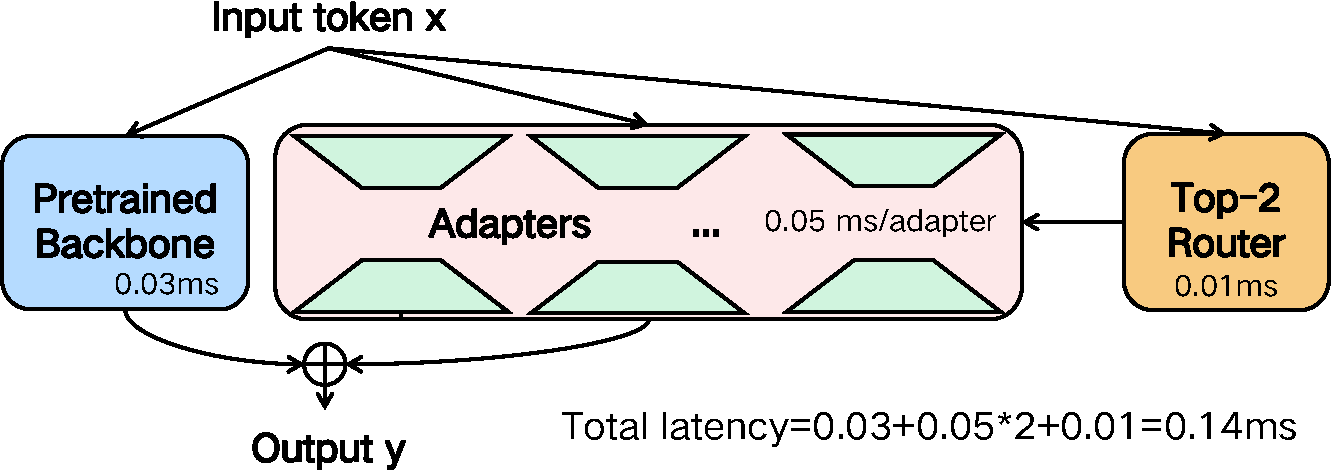
\includegraphics[width=0.95\columnwidth]{figures/adapter_latency.pdf}
    \caption{Decoding phase execution time profiling of one dynamic adapter layer in MoRAL. The execution time results were preceded by a warm-up of 100 executions and are obtained on the average of 300 executions.}
    \label{fig:cuda_launch}
\end{figure}

To elucidate the sources of latency overhead introduced by dynamic adapters, we conducted a granular analysis of latency within various components during the decoding phase. As illustrated in Figure~\ref{fig:cuda_launch}, it is evident that the execution time for the adapters (0.05ms) exceeds that of the pretrained backbone (0.03ms). Despite the relatively modest computational complexity of the LoRA adapters employed in dynamic configurations, each adapter necessitates dual launches of CUDA kernel context operations. The execution time of these CUDA kernels does not correlate linearly with the size of the matrices involved, leading to considerable latency in the adapter components.

\noindent\noindent\textbf{In-depth Latency Profiling.} To meticulously investigate how the inference latency of LoRA adapters and the pretrained backbone varies with increasing computational demands, we conducted tests across different input sequence lengths and examined the relationship between adapter rank and inference latency.

As shown in Figure~\ref{figure:detailed adapter profiling}, regardless of whether it is during the prefilling or decoding phase, and irrespective of the LoRA ranks being high or low, the latency of the LoRA adapters consistently exceeds that of the backbone. This phenomenon is primarily attributed to the number of CUDA kernel calls rather than the computing complexity involved in each call. The underlying reason is that the latency associated with CUDA kernel calls does not scale linearly with computing complexity. This insight highlights a crucial aspect of system behavior that significantly impacts the performance of dynamic adapters.

\begin{figure}[!h]
    \centering
    \begin{subfigure}[b]{0.45\textwidth}
        \centering
        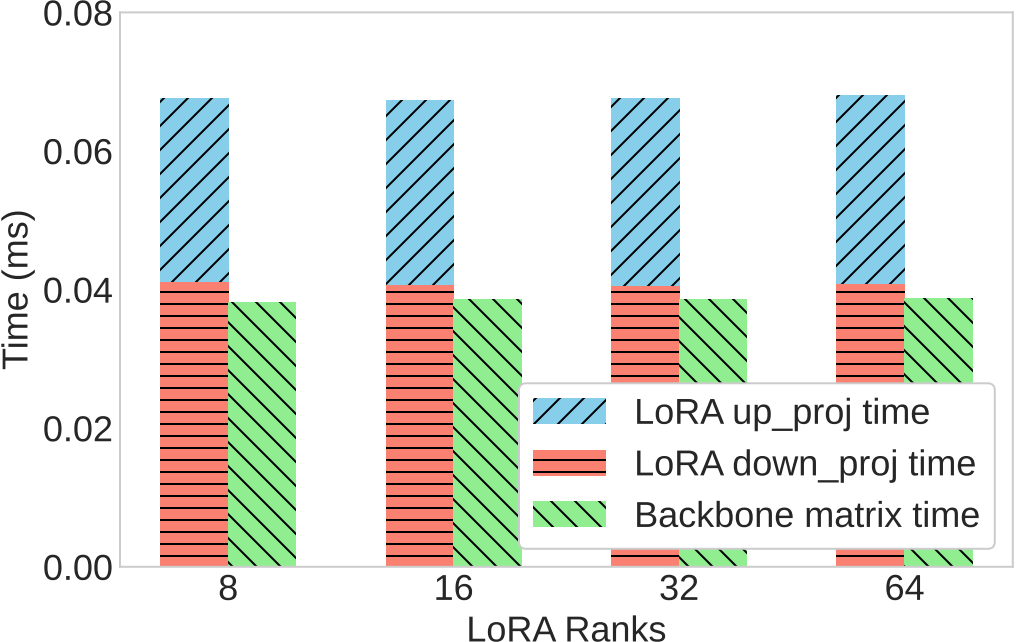
\includegraphics[width=\textwidth]{figures/lora_vs_backbone_time_100_token_lqy.png}
        \caption{Prefilling phase: sequence length is 100.}
    \end{subfigure}
    \begin{subfigure}[b]{0.45\textwidth}
        \centering
    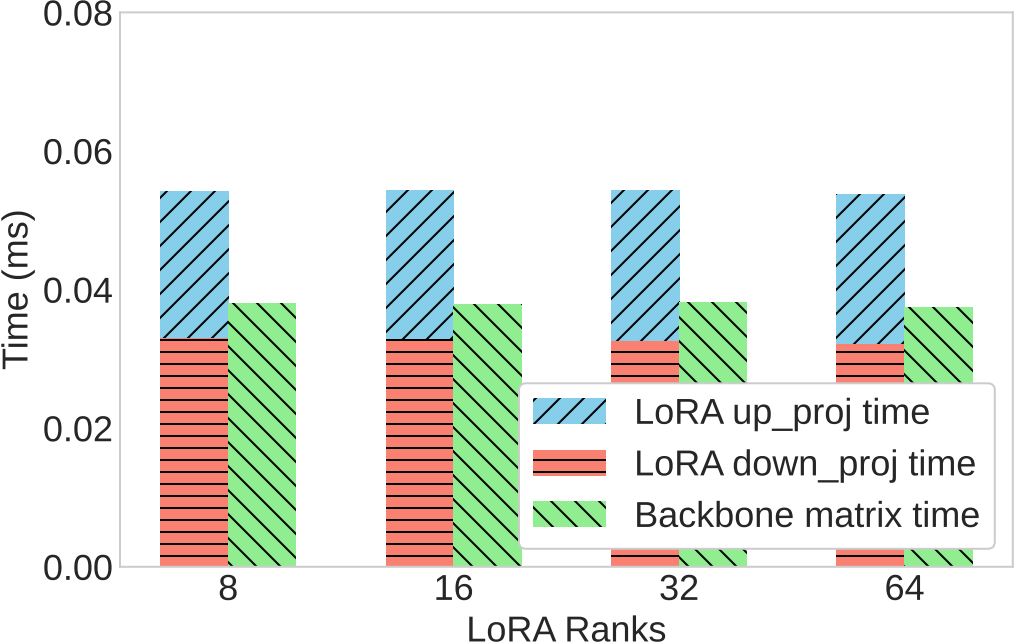
\includegraphics[width=\textwidth]{figures/lora_vs_backbone_time_1_token_lqy.png}
        \caption{Decoding phase: sequence length is 1.}
    \end{subfigure}
    \caption{Latency breakdown of one dynamic adapter layer under different settings.}
    \label{figure:detailed adapter profiling}
\end{figure}

% \subsection{Challenge of Reducing Latency Overhead}
\noindent\noindent\textbf{Challenge of Reducing Latency Overhead.}
A straightforward way to reduce inference latency overhead is to reduce the times of CUDA kernel context operations. Like LoRA~\cite{Hu2021LoRALA}, one could pre-merge adapters into the original matrix and then perform token decoding computation. We use this simple strategy in MoRAL by directly merging activated adapters layer by layer before computing. However, the additional operations introduced higher latency, where the decoding latency is 4.5 ms/token, which is still 88\% higher than the original LLM model. This is because merging a LoRA adapter into the backbone matrix requires an additional invocation of a CUDA kernel to perform the matrix multiplication for the up and down projections.
